
\section{Dữ liệu 4}
Bộ dữ liệu ghi lại những yếu tố có thể ảnh hưởng đến lương (\$ giờ) của người lao động ở Anh năm 1976.

\subsection*{Tìm hiểu dữ liệu}
Bộ dữ liệu gồm 13 biến sau:
\begin{itemize}
	\item \texttt{wage}: Số lượng trung bình một giờ
	\item \texttt{educ}: Số năm đào tạo
	\item \texttt{exper}: Số năm kinh nghiệm tiềm năng
	\item \texttt{tenure}: Số năm làm việc hiện tại
	\item \texttt{nonwhite}: 1 nếu là người da màu
	\item \texttt{female}: 1 nếu là phụ nữ
	\item \texttt{married}: 1 nếu đã kết hôn
	\item \texttt{numdep}: Số người phụ thuộc
	\item \texttt{smsa}: 1 nếu sống ở vùng đô thị Hoa Kỳ
	\item \texttt{northcen}: 1 nếu sống ở phía Bắc trung tâm Hoa Kỳ
	\item \texttt{south}: 1 nếu sống ở khu vực phía Nam
	\item \texttt{west}: 1 nếu sống ở khu vực phía Tây
	\item \texttt{construc}: 1 nếu làm việc ở construc. indus
	\item \texttt{ndurman}: 1 nếu làm việc nondur. manuf. indus.
	\item \texttt{trcommpu}: 1 nếu trong trans, commun, pub ut
	\item \texttt{trade}: 1 nếu bán buôn hoặc bán lẻ
	\item \texttt{services}: 1 nếu trong services indus.
	\item \texttt{profserv}: 1 nếu trong prof. serv. indus.
	\item \texttt{profocc}: 1 nếu trong profess. occupation
	\item \texttt{clerocc}: 1 nếu trong clerical occupation
	\item \texttt{servocc}: 1 nếu trong service occupation
	\item \texttt{lwage}: \texttt{log(wage)}
	\item \texttt{expersq}: \texttt{exper2}
	\item \texttt{tenursq}: \texttt{tenure2}
\end{itemize}

\begin{figure}[H]
	\centering
	{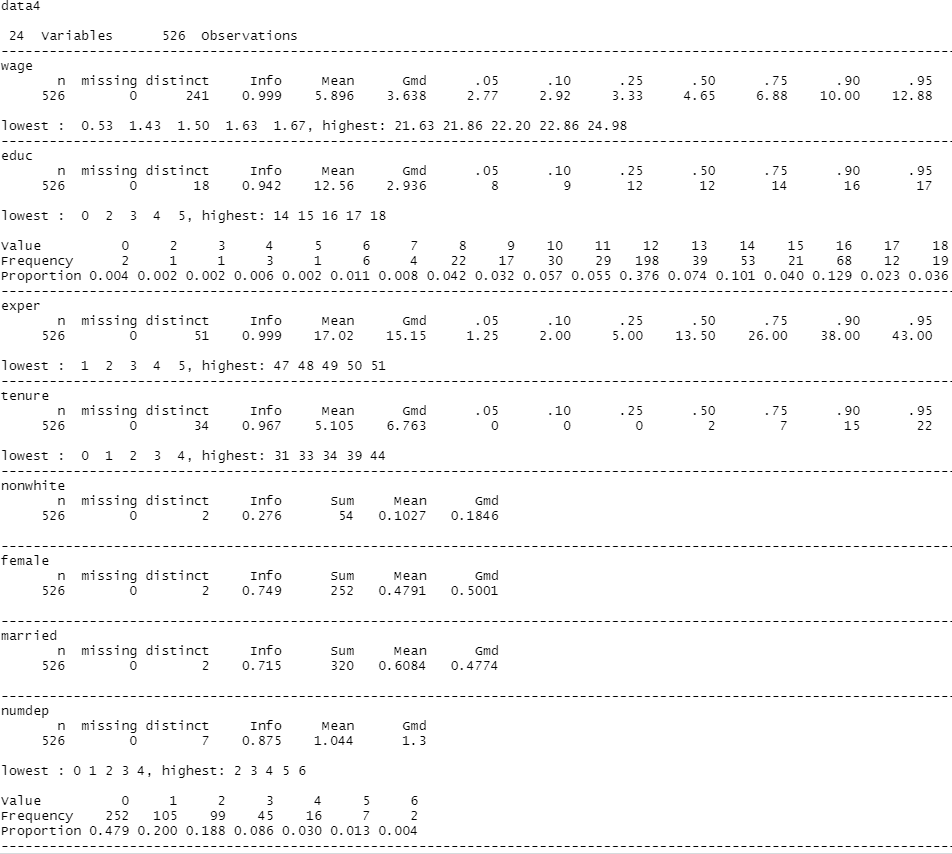
\includegraphics[width=0.63\linewidth]{../Photo Of Result/describe(4)-1}}
\end{figure}
\begin{figure}[H]
	\centering
	{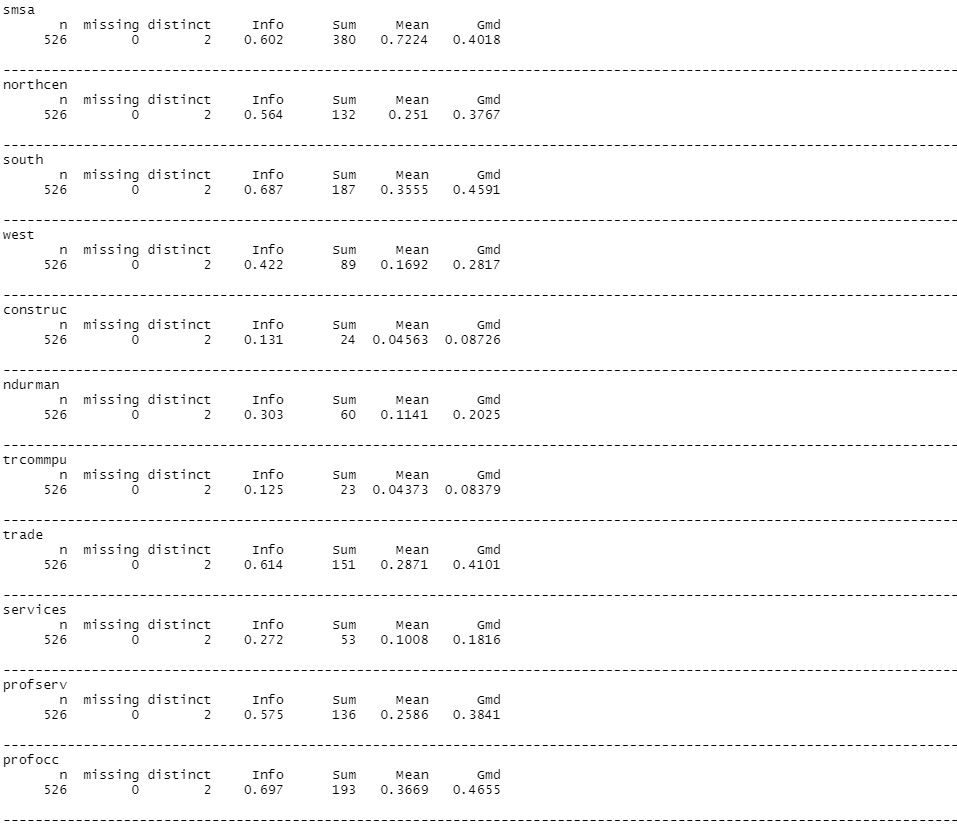
\includegraphics[width=0.63\linewidth]{../Photo Of Result/describe(4)-2}}
	{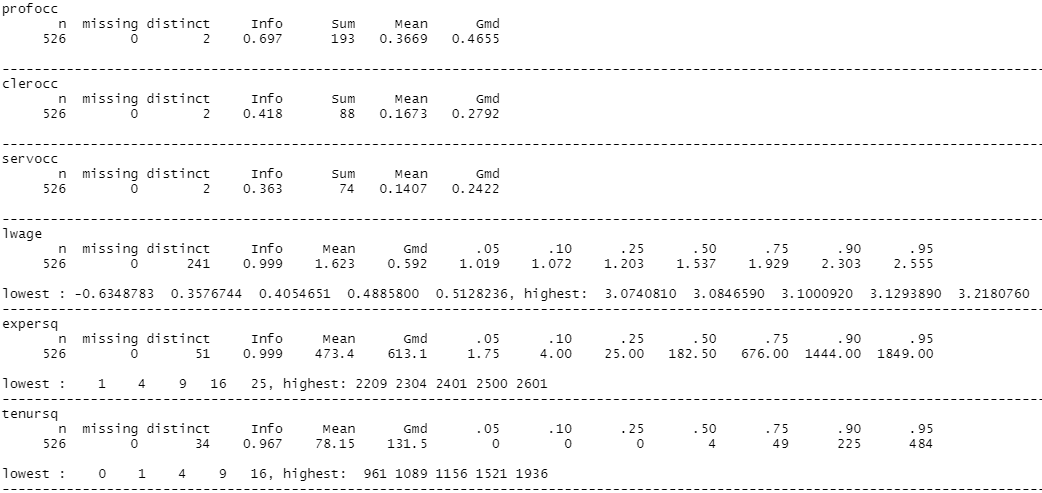
\includegraphics[width=0.63\linewidth]{../Photo Of Result/describe(4)-3}}
	\caption{Khái quát dữ liệu}
	\label{describe-4}
\end{figure}

Dựa vào kết quả mô tả dữ liệu từ R trong hình \ref{describe-4}, ta thấy được bộ dữ liệu gồm  24 biến và 526 quan trắc, các biến dữ liệu không bị missing value và được chia làm hai loại:
\begin{itemize}
	\item Các biến định tính: \texttt{nonwhite}, \texttt{female}, \texttt{married}, \texttt{smsa}, \texttt{northcen}, \texttt{south}, \texttt{west}, \texttt{construc}, \texttt{ndurman}, \texttt{trcommpu}, \texttt{trade}, \texttt{services}, \texttt{profserv}, \texttt{profocc}, \texttt{clerocc}, \texttt{servocc}.
	\item Các biến định lượng: \texttt{wage}, \texttt{educ}, \texttt{exper}, \texttt{tenure}, \texttt{numdep}, \texttt{lwage}, \texttt{expersq}, \texttt{tenursq}.
\end{itemize}

\subsection*{Phân tích dữ liệu}
\begin{figure}[H]
	\centering
	\subfloat[Biểu đồ biến định lượng theo độ tương quan, sơ đồ cột, điểm dữ liệu]
	{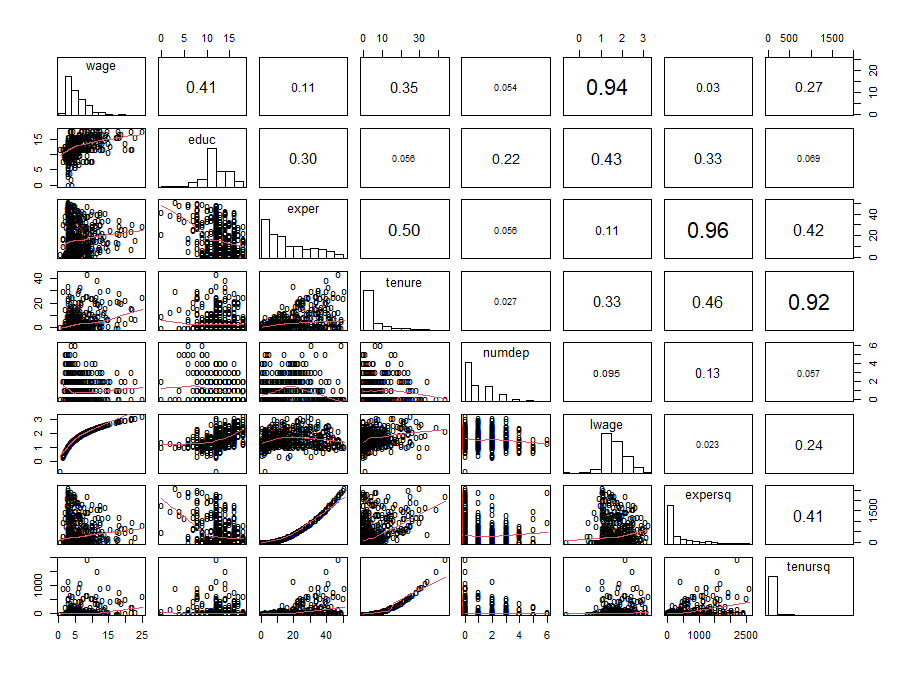
\includegraphics[width=0.8\textwidth]{../Photo Of Result/Plot-dinhluong-data4}} \hfill
	\subfloat[Biểu đồ biến định tính theo độ tương quan, sơ đồ cột, điểm dữ liệu]
	{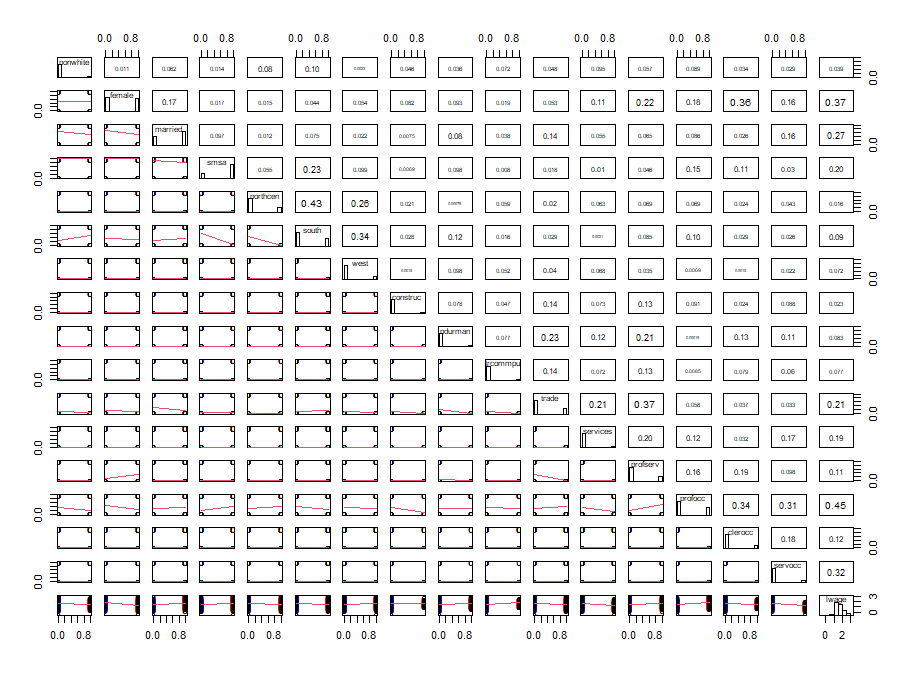
\includegraphics[width=0.85\textwidth]{../Photo Of Result/Plot-dinhtinh-data4}}
	\caption{Biểu đồ vẽ các biến theo độ tương quan, sơ đồ cột, điểm dữ liệu}
	\label{plot_data4}
\end{figure}

Dựa vào hình \ref{plot_data4}, ta thấy độ tương quan giữa ba cặp biến (\texttt{lwage}, \texttt{wage}), (\texttt{tenursq}, \texttt{tenure}, (\texttt{expersq}, \texttt{exper}) đều trên $0.9$ nên ta sẽ phải bỏ ba biến này ra khỏi bộ dữ liệu để tránh hiện tượng đa cộng tuyến. Nhìn vào bộ dữ liệu, ta nhận thấy được các biến \texttt{lwage}, \texttt{tenursq}, \texttt{expersq} đều là sự biến đổi từ ba biến \texttt{wage}, \texttt{tenure}, \texttt{exper} ban đầu nên ta sẽ quyết định bỏ hẳn 3 biến \texttt{lwage}, \texttt{tenursq}, \texttt{expersq} này ra khỏi bộ dữ liệu.

\subsection*{Chọn mô hình}

Ta sẽ xây dựng mô hình hồi quy tuyến tính đầy đủ:

\begin{figure}[H]
	\centering
	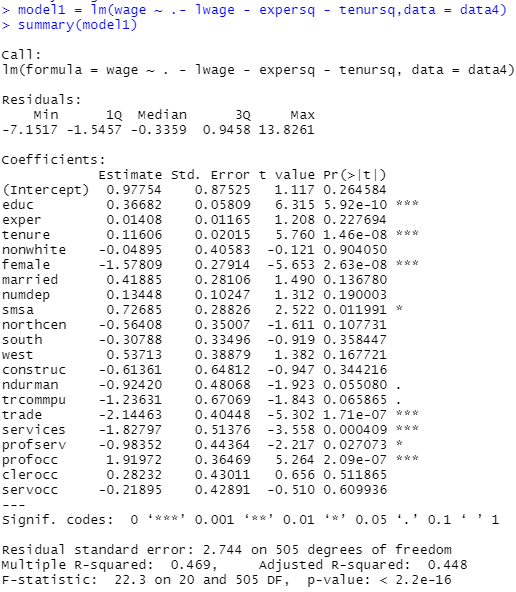
\includegraphics[width=0.7\textwidth]{../Photo Of Result/full-model-data4}
	\caption{Kết quả hồi quy mô hình đầy đủ từ R}
	\label{full-model}
\end{figure}

Ta có thể thấy trong hình \ref{full-model} chỉ một vài biến như là \texttt{educ}, \texttt{tenure}, \texttt{female}, \texttt{trade}, \texttt{services}, \texttt{profocc} có ý nghĩa thống kê $0.001$. Do đó, ta cần sử dụng các phương pháp chọn biến để mô hình tốt hơn.

\subsubsection*{Hướng tiếp cận 1: Chọn tất cả}

\begin{longtable}{cllll}
	\hline
	\begin{tabular}[c]{@{}c@{}}Số lượng \\ biến\end{tabular} &
	\multicolumn{1}{c}{Biến dự đoán} &
	\multicolumn{1}{c}{$R^2_{adj}$} &
	\multicolumn{1}{c}{$C_p$} &
	\multicolumn{1}{c}{BIC} \\ \hline
	\endhead
	%
	\hline
	\endfoot
	%
	\endlastfoot
	%
	1 &
	profocc &
	\multicolumn{1}{c}{0.19362} &
	243.45475 &
	-101.6706 \\
	2 &
	educ, tenure &
	\multicolumn{1}{c}{0.29919} &
	143.97580 &
	-170.2154 \\
	3 &
	educ, tenure, female &
	\multicolumn{1}{c}{0.35396} &
	92.91189 &
	-207.7622 \\
	4 &
	educ, tenure, female, profocc &
	0.39249 &
	57.37900 &
	-234.8483 \\
	5 &
	educ, tenure, femanle, profocc, trade &
	0.41818 &
	34.07821 &
	-252.3208 \\
	6 &
	educ, tenure, female, profocc, trade, west &
	0.42657 &
	27.14121 &
	-254.7032 \\
	7 &
	\begin{tabular}[c]{@{}l@{}}educ, tenure, female, profocc, trade, west, \\ services\end{tabular} &
	0.43425 &
	20.89218 &
	-256.5481 \\
	8 &
	\begin{tabular}[c]{@{}l@{}}educ, tenure, female, profocc, trade, west,\\ services, smsa\end{tabular} &
	0.44033 &
	16.16804 &
	\textbf{-256.9875} \\
	9 &
	\begin{tabular}[c]{@{}l@{}}educ, tenure, female, profocc, trade, west,\\ services, smsa, married\end{tabular} &
	0.44469 &
	13.08489 &
	-255.8480 \\
	10 &
	\begin{tabular}[c]{@{}l@{}}educ, tenure, female, profocc, trade, west,\\ services, smsa, married, northcen\end{tabular} &
	0.44560 &
	13.22747 &
	-251.4683 \\
	11 &
	\begin{tabular}[c]{@{}l@{}}educ, tenure, female, profocc, trade, west,\\ services, smsa, married, ndurman, profserv\end{tabular} &
	0.44637 &
	13.50318 &
	-246.9594 \\
	12 &
	\begin{tabular}[c]{@{}l@{}}educ, tenure, female, profocc, trade, west,\\ services, smsa, married, ndurman, profserv,\\ trcommpu\end{tabular} &
	0.44827 &
	12.73335 &
	-243.5280 \\
	13 &
	\begin{tabular}[c]{@{}l@{}}educ, tenure, female, profocc, trade, west, \\ services, smsa, married, ndurman, profserv, \\ trcommpu, northcen\end{tabular} &
	0.44939 &
	12.69999 &
	-239.3528 \\
	14 &
	\begin{tabular}[c]{@{}l@{}}educ, tenure, female, profocc, trade, west,\\ services, smsa, married, ndurman, profserv,\\ trcommpu, northcen, numdep\end{tabular} &
	0.44959 &
	13.51543 &
	-234.3090 \\
	15 &
	\begin{tabular}[c]{@{}l@{}}educ, tenure, female, profocc, trade, west,\\ services, smsa, married, ndurman, profserv, \\ trcommpu, northcen, numdep, exper\end{tabular} &
	\textbf{0.45032} &
	13.84069 &
	-229.7754 \\
	16 &
	\begin{tabular}[c]{@{}l@{}}educ, tenure, female, profocc, trade, west,\\ services, smsa, married, ndurman, profserv,\\ trcommpu, nothcen, numdep, exper, south\end{tabular} &
	0.45015 &
	15.00327 &
	-224.3782 \\
	17 &
	\begin{tabular}[c]{@{}l@{}}educ, tenure, female, profocc, trade, west,\\ services, smsa, married, ndurman, profserv, \\ trcommpu, northcen, numdep, exper, construc,\\ clerocc\end{tabular} &
	0.45003 &
	16.12009 &
	-219.0300 \\
	18 &
	\begin{tabular}[c]{@{}l@{}}educ, tenire, female, profocc, trade, west,\\ services, smsa, married, ndurman, profserv, \\ trcommpu, northcen, numdep, exper, construc, \\ clerocc, south\end{tabular} &
	0.44988 &
	17.26616 &
	-213.6529 \\
	19 &
	\begin{tabular}[c]{@{}l@{}}educ, tenire, female, profocc, trade, west,\\ services, smsa, married, ndurman, profserv, \\ trcommpu, northcen, numdep, exper, construc,\\ clerocc, south, servocc\end{tabular} &
	0.44906 &
	\textbf{19.01455} &
	-207.6496 \\
	20 &
	\begin{tabular}[c]{@{}l@{}}educ, tenire, female, profocc, trade, west,\\ services, smsa, married, ndurman, profserv, \\ trcommpu, northcen, numdep, exper, construc,\\ clerocc, south, servocc, nonwhite\end{tabular} &
	0.44799 &
	21.00000 &
	-201.3995 \\ \hline
	\caption{Giá trị $R^2_{adj}$, $C_p$, BIC, cho từng tập biến con tốt nhất}
	\label{table-all-subset}\\
\end{longtable}

Dựa vào bảng \ref{table-all-subset} ta thấy được mô hình có chỉ số BIC tốt nhất là mô hình 8 biến. Tuy nhiên mô hình có hệ số xác định hiệu chỉnh tốt nhất là mô hình có 15 biến và mô hình có hệ số $C_p$ tốt nhất là mô hình 19 biến dự đoán.


\subsubsection*{Hướng tiếp cận 2: Phương pháp tiến dựa trên AIC}
\begin{figure}[H]
	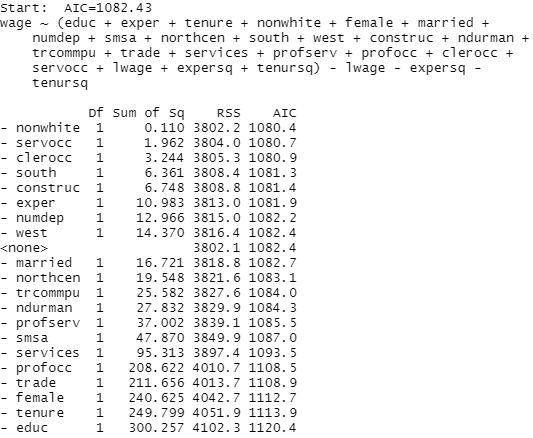
\includegraphics[width=0.45\textwidth]{../Photo Of Result/stepAIC(4)-1}
	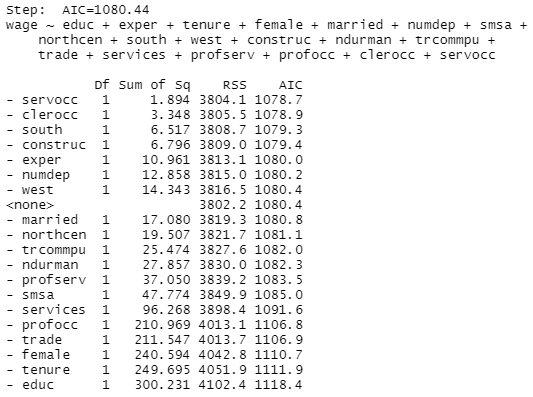
\includegraphics[width=0.45\textwidth]{../Photo Of Result/stepAIC(4)-2}
	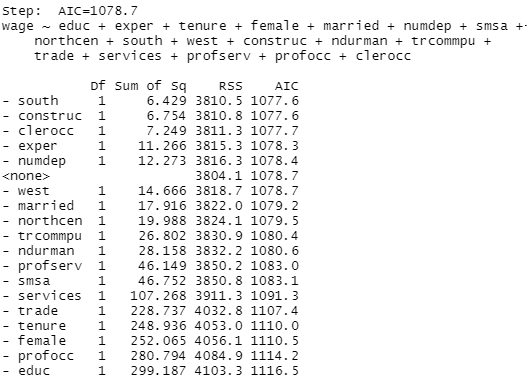
\includegraphics[width=0.45\textwidth]{../Photo Of Result/stepAIC(4)-3}
	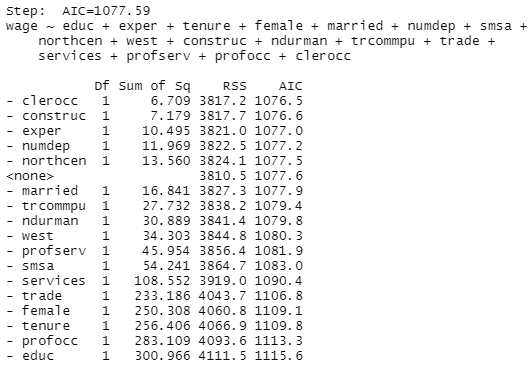
\includegraphics[width=0.45\textwidth]{../Photo Of Result/stepAIC(4)-4}
	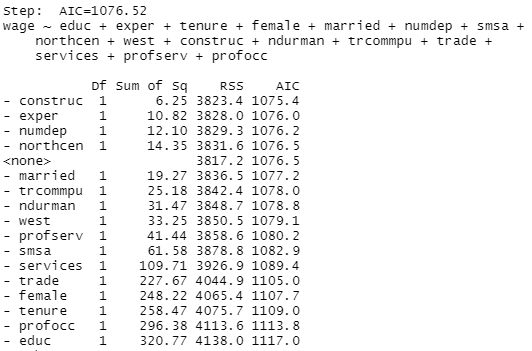
\includegraphics[width=0.45\textwidth]{../Photo Of Result/stepAIC(4)-5}
	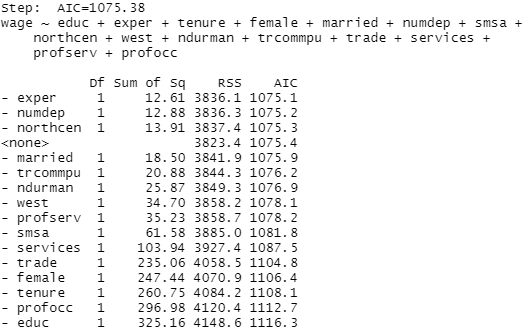
\includegraphics[width=0.45\textwidth]{../Photo Of Result/stepAIC(4)-6}
	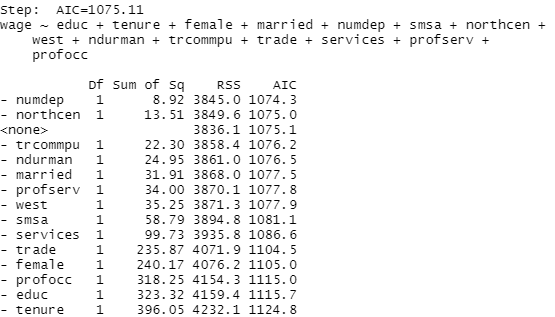
\includegraphics[width=0.45\textwidth]{../Photo Of Result/stepAIC(4)-7}
	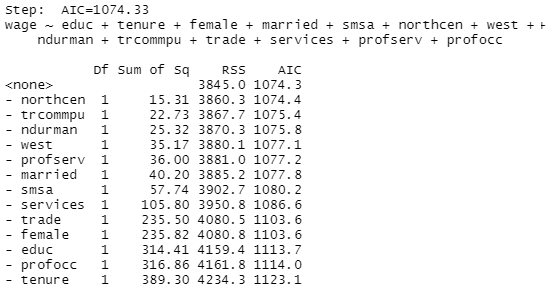
\includegraphics[width=0.45\textwidth]{../Photo Of Result/stepAIC(4)-8}
	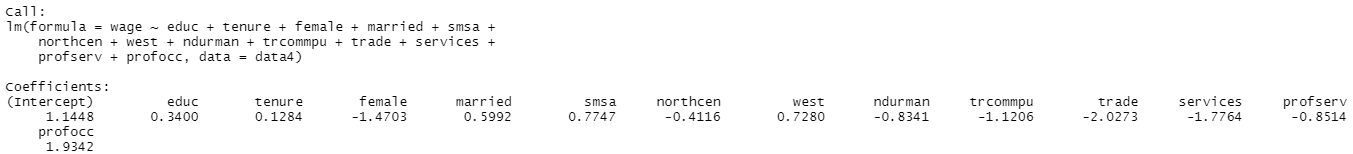
\includegraphics[width=\textwidth]{../Photo Of Result/stepAIC(4)-9}
	\caption{Các biến định tính được vẽ ra}
	\label{stepAIC}
\end{figure}

Dựa vào hình \ref{stepAIC}, sau khi chạy code R phương pháp lùi dựa theo tiêu chí AIC thì mô hình chọn được là mô hình gồm 11 biến:

\begin{equation*}
	\begin{multlined}
		\texttt{wage } = \beta_0 + \text{ } \beta_{educ}\times \texttt{educ} \text{ } + \text{ } \beta_{tenure} \times \texttt{tenure} \text{ }+\text{ }\beta_{female} \times \texttt{female} \text{ } \\
		+ \beta_{married} \text{ } \times \texttt{married} \text{ } +\text{ }\beta_{smsa} \times\texttt{smsa}\text{ } +\text{ }\beta_{northcen}\times \texttt{northcen} \\
		+\text{ }\beta_{west} \times \texttt{west} \text{ } + \text{ }\beta_{ndurman}\times \texttt{ndurman}\text{ } +\text{ }\beta_{trcommpu} \times\texttt{trcommpu}\text{ } \\
		+\text{ }\beta_{trade}\times \texttt{trade} +\text{ }\beta_{services} \times \texttt{services} \text{ } 
		+ \text{ }\beta_{profserv} \times \texttt{profserv} \text{ } + \text{ }\beta_{profocc}\times \texttt{profocc}
	\end{multlined}
\end{equation*}

\subsubsection*{Hướng tiếp cận 3: Phương pháp Stagewise}
\begin{figure}[H]
	\centering
	\subfloat[Biểu đồ chọn mô hình hồi quy]
	{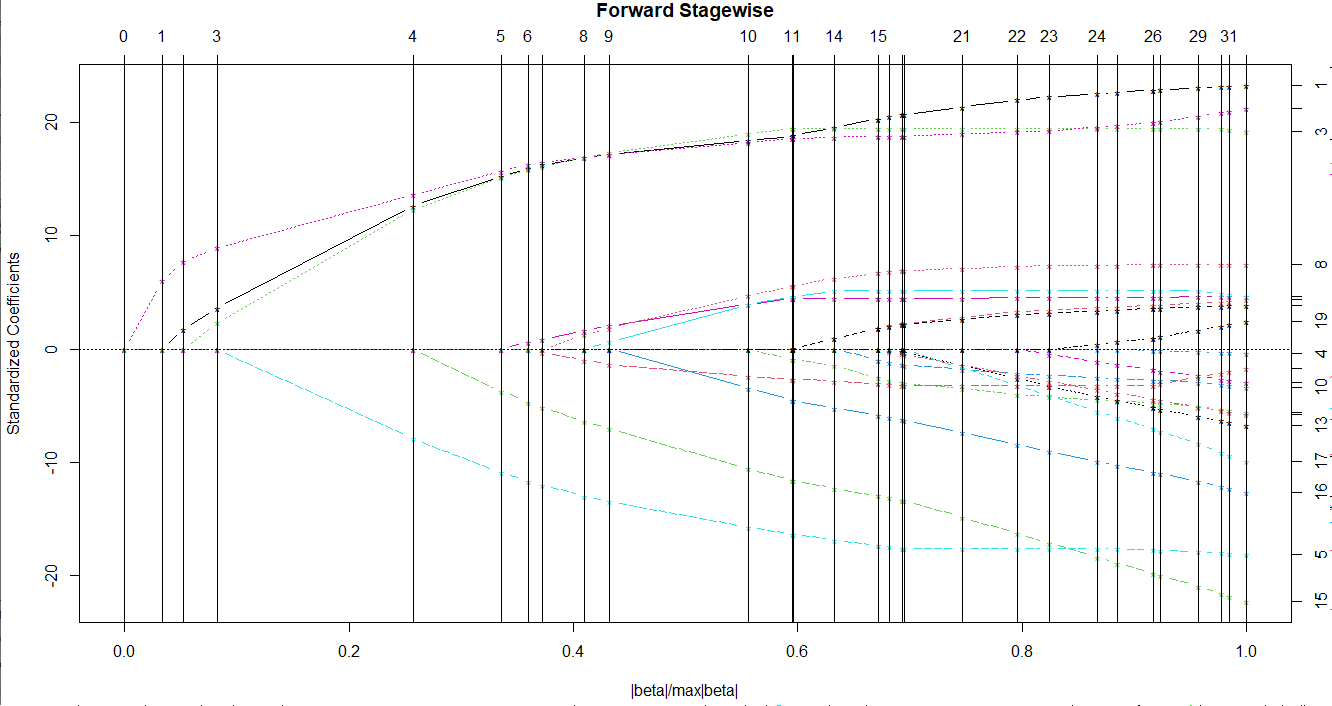
\includegraphics[width=.7\linewidth]{../Photo Of Result/stagewise plot}} \hfill
	\subfloat[Bảng hệ số của mô hình hồi quy]
	{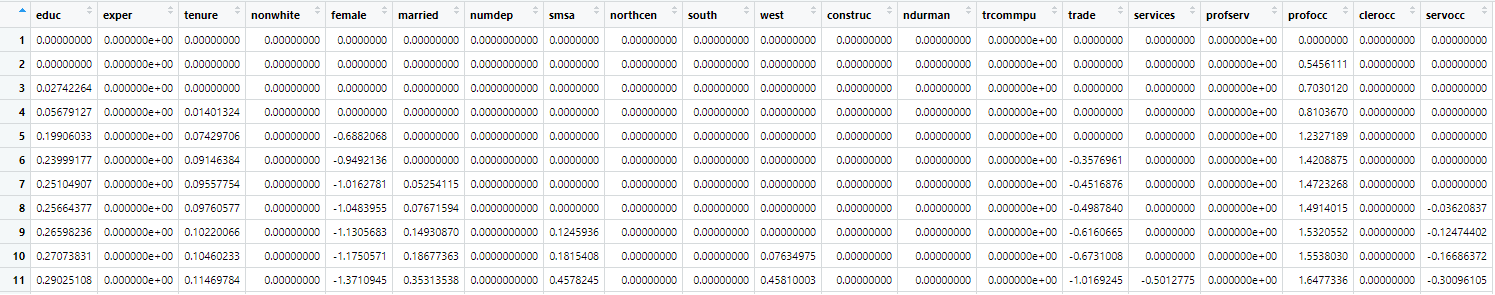
\includegraphics[width=.8\linewidth]{../Photo Of Result/coef-stagewise-4}}
	\caption{Biểu đồ Stagewise cho mô hình hồi quy}
	\label{stagewise}
\end{figure}

Dựa vào hình \ref{stagewise}, sau khi chạy code R, phương pháp Stagewise đưa ra đề xuất model gồm 11 biến:

\begin{equation*}
	\begin{multlined}
		\texttt{wage } = \beta_0 + \text{ } \beta_{educ}\times \texttt{educ} \text{ } + \text{ } \beta_{tenure} \times \texttt{tenure} \text{ }+\text{ }\beta_{female} \times \texttt{female} \text{ } 
		+ \beta_{married} \text{ } \times \texttt{married} \text{ } \\
		+\text{ }\beta_{smsa} \times\texttt{smsa}\text{ }  
		+ \text{ }\beta_{west} \times \texttt{west} \text{ } 
		+ \text{ }\beta_{trade}\times \texttt{trade} + \text{ }\beta_{services} \times \texttt{services} \text{ } \\
		+ \text{ }\beta_{servocc} \times \texttt{servocc} \text{ } + \text{ }\beta_{profocc}\times \texttt{profocc}
	\end{multlined}
\end{equation*}

Dựa vào cả ba hướng tiếp cận, ta sẽ xây dựng 5 mô hình hồi quy lại theo các phương pháp chọn biến:

\begin{figure}[H]
	\begin{tabular}{cc}
		\centering
		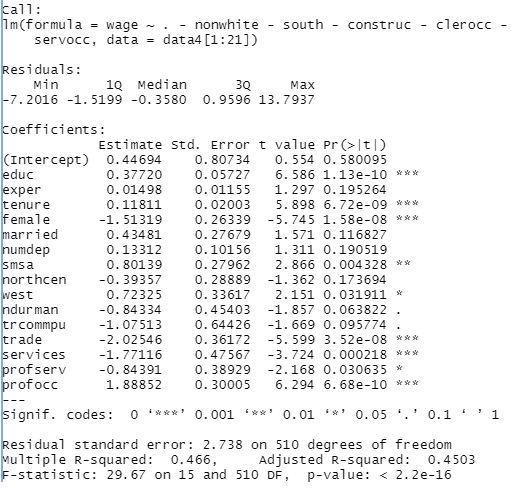
\includegraphics[width=0.4\textwidth]{../Photo Of Result/model-R-4} &   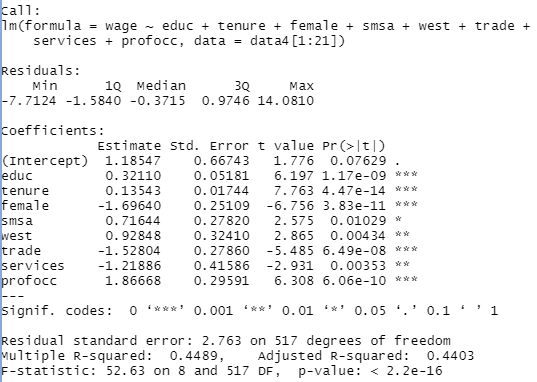
\includegraphics[width=0.45\textwidth]{../Photo Of Result/model-BIC-4} \\
		(a) Mô hình hồi quy theo giá trị $R^2_{adj}$  & (b) Mô hình hồi quy theo giá trị BIC \\[6pt]
		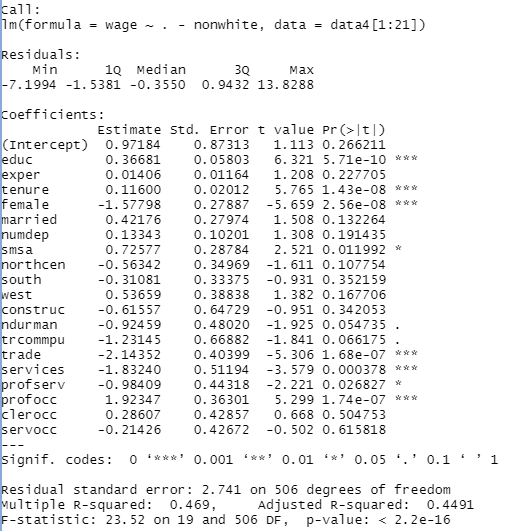
\includegraphics[width=0.45\textwidth]{../Photo Of Result/model-Cp-4} &   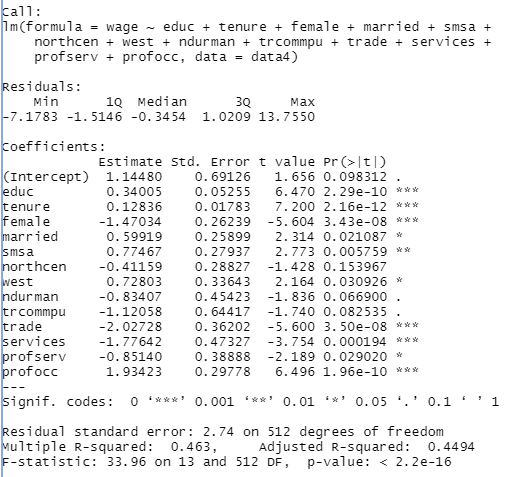
\includegraphics[width=0.45\textwidth]{../Photo Of Result/model-stepwise-aic-4} \\
		(c) Mô hình hồi quy theo giá trị $C_p$ & (d) Mô hình hồi quy Stepwise dựa trên AIC \\[6pt]
		\multicolumn{2}{c}{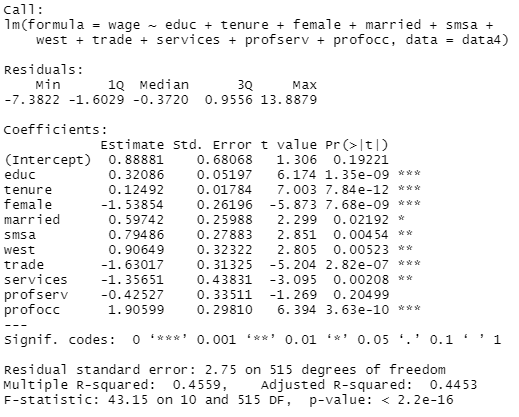
\includegraphics[width=0.45\textwidth]{../Photo Of Result/model-stagewise-4} }\\
		\multicolumn{2}{c}{(e) Mô hình hồi quy theo phương pháp Stagewise}
	\end{tabular}
	\caption{Mô hình hồi quy dựa trên các phương pháp chọn biến}
	\label{5-model-reg}
\end{figure}

Dựa vào kết quả R trong hình \ref{5-model-reg}, ta chọn mô hình gồm 8 biến theo phương pháp chọn tất cả dựa vào chuẩn BIC. Tuy nhiên, các hệ số hồi quy vẫn chưa đạt được mức ý nghĩa thống kê $0.05$ nên ta sẽ biến đổi log biến được giải thích $wage$ thành biến $lwage$, và xây dựng lại mô hình dựa trên 8 biến được chọn ra.

\begin{equation*}
	\begin{multlined}
		\texttt{lwage } = \beta_0 + \text{ } \beta_{educ}\times \texttt{educ} \text{ } + \text{ } \beta_{tenure} \times \texttt{tenure} \text{ }+\text{ }\beta_{female} \times \texttt{female} \text{ } \\
		+\text{ }\beta_{smsa} \times\texttt{smsa}\text{ }  
		+ \text{ }\beta_{west} \times \texttt{west} \text{ } 
		+ \text{ }\beta_{trade}\times \texttt{trade} + \text{ }\beta_{services} \times \texttt{services} \text{ }\\ + \text{ }\beta_{profocc}\times \texttt{profocc}
	\end{multlined}
\end{equation*}


\begin{figure}[H]
	\centering
	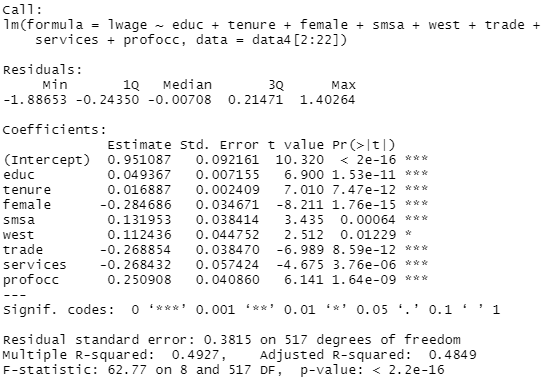
\includegraphics[width=0.7\textwidth]{../Photo Of Result/model-final-4}
	\caption{Mô hình hồi quy với 8 biến được chọn và đã qua chuẩn hóa log}
	\label{model-final-4}
\end{figure}

Dựa vào kết quả trong hình \ref{model-final-4}, ta được mô hình hồi quy:
\begin{equation*}
\begin{multlined}
	\texttt{lwage } = \text{ } 0.0493\times \texttt{educ} \text{ } + \text{ } 0.0169 \times \texttt{tenure} \text{ }-\text{ }0.2846 \times \texttt{female} \text{ } + 0.1319 \text{ } \times \texttt{smsa} \text{ } \\
	+\text{ }0.1124 \times\texttt{west}\text{ } -\text{ }0.2689\times \texttt{trade} -\text{ }0.2684 \times \texttt{services} \text{ } + \text{ }0.2509\times \texttt{profocc} + 0.951
\end{multlined}
\end{equation*}

\begin{figure}[H]
	\centering
	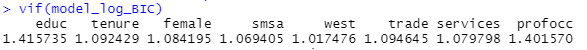
\includegraphics[width=\textwidth]{../Photo Of Result/vif-4}	
	\caption{Hệ số VIF của mô các biến được chọn}
	\label{vif}
\end{figure}

Từ kết quả chạy từ R trong hình \ref{vif}, ta thấy được mô hình không vi phạm điều kiện nào của mô hình tuyến tính. Trong mô hình không tồn tại hiện tượng đa cộng tuyến (VIF < 5.0).

\begin{figure}[H]
	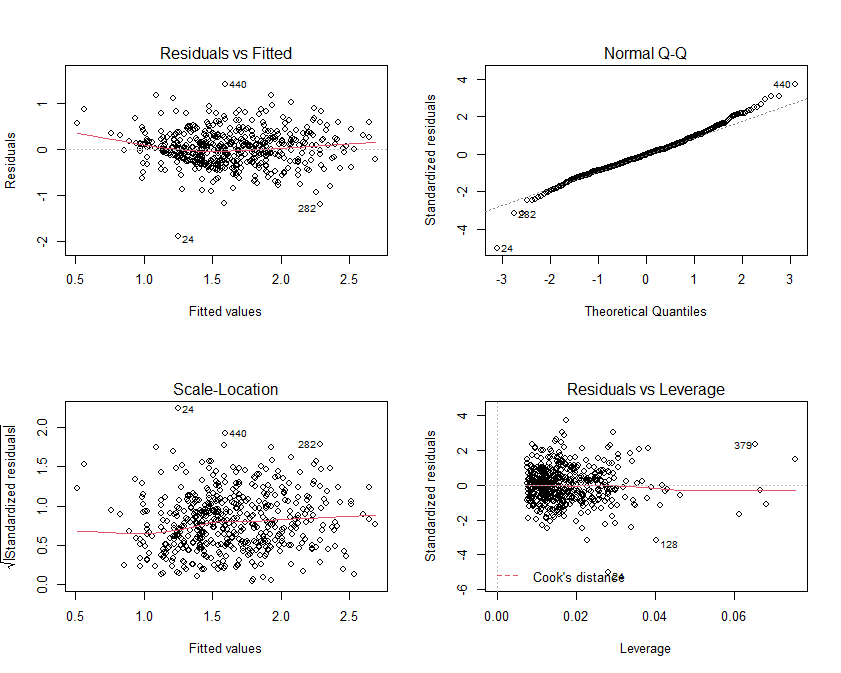
\includegraphics[width=\textwidth]{../Photo Of Result/diagnostic-plot-4}
	\caption{Các biểu đồ đánh giá mô hình}
	\label{diagnostic}
\end{figure}

Dựa vào hình \ref{diagnostic} (Normal Q-Q), ta có thể thấy được các điễm nằm gần như trên đường chéo, tức là sai số có phương sai không đổi và đã tuân theo phân phối chuẩn.

\subsection*{Kết luận}
Khi kiểm tra các giả thiết ý nghĩa của mô hình:
\begin{itemize}
	\item Vấn đề đa cộng tuyến trong bộ dữ liệu xảy ra rất nhiều, nhưng khi sử dụng các phương pháp chọn biến thì đã vô tình loại bỏ được hiện tượng đa cộng tuyến.
	\item Phần dư $\epsilon$ trong mô hình chọn tuân theo phân phối chuẩn.
\end{itemize}
Mô hình được chọn có ý nghĩa thống kê gồm 8 biến với hệ số xác định hiệu chỉnh $0.4849$, tức là mô hình được lựa chọn chỉ giải thích được khoảng $49\%$ bộ dữ liệu. Ta có thấy được mức lương được ảnh hưởng nhiều bởi biến giới tính, biến về vị trí; các biến về số năm đào tạo, số năm làm việc không ảnh hưởng gì nhiều đến mức lương.

Tuy nhiên, việc chọn mô hình này không hiệu quả vì chỉ giải thích được dưới $50\%$ bộ dữ liệu này. Với bộ dữ liệu này, nên cân nhắc một phương pháp mới phức tạp hơn để dự đoán giá lương chứ không đơn thuần chỉ sử dụng mô hình hồi quy tuyến tính.
